\section{Resultados e discussões}
\subsection{Pêndulo de Wilberforce}
Neste experimento, foi analisado o comportamento do Pêndulo de Wilberforce, um sistema que exemplifica de forma clara o fenômeno de oscilações acopladas. O aspecto mais notável do pêndulo é a transferência gradual de energia entre os modos de oscilação longitudinal e rotacional, resultando em alternâncias periódicas entre esses movimentos.

A origem dessa transferência de energia está no acoplamento entre os dois modos de oscilação, causado pelas propriedades geométricas e elásticas da mola. Quando a massa oscila verticalmente, a mola se comprime e se estende. Devido à sua estrutura helicoidal, essas variações induzem uma torção no sistema, influenciando o movimento rotacional. Esse acoplamento permite que a energia seja transferida entre os modos de oscilação, caracterizando o sistema como um oscilador acoplado .

Para que a transferência de energia entre os modos longitudinal e rotacional seja eficiente, é fundamental que suas frequências naturais sejam próximas. Uma forma de ajustar essa proximidade é modificando a frequência do modo rotacional por meio da posição dos discos laterais, o que altera o momento de inércia da massa suspensa. Quando essa condição é atingida, o sistema pode entrar em ressonância, o que favorece a troca contínua de energia entre os dois modos de oscilação.

Durante esse processo, a energia potencial elástica associada à compressão e extensão da mola (modo longitudinal) e a energia potencial de torção (modo rotacional) são convertidas em suas respectivas formas de energia cinética. A energia cinética translacional está relacionada ao movimento vertical da massa, enquanto a energia cinética rotacional está associada à sua rotação. A alternância entre esses modos resulta em uma oscilação da amplitude de cada movimento, evidenciando a transferência gradual de energia no sistema.

Esse comportamento do Pêndulo de Wilberforce não apenas ilustra princípios fundamentais da física de oscilações acopladas, mas também encontra analogias em sistemas do cotidiano, como a maquina de lavar. Uma vez que, como um pêndulo de Wilberforce, ela realiza oscilações no 
eixo rotacional e oscilações no eixo longitudinal. Essa dinâmica de um oscilador acoplado, lhe confere a propriedade de transferência 
gradual de energia entre os modos de oscilação, e dependência da ressonância entre as oscilações para melhor funcionamento do equipamento.
Dessa forma, se a frequência da rotação estiver muito descalibrada, devido ao acumulo de massa em um ponto do cesto da máquina por exemplo,
pode ocasionar em um transferência excessiva de energia para a oscilação longitudinal, o que pode danificar o máquina.

\subsection{Pêndulo de Torção}  

Para analisar o comportamento do pêndulo de torção em diferentes meios, foi medido o tempo necessário para realizar oscilações tanto no 
ar quanto no óleo. Dessas medições, pontuou-se as 5 primeiras oscilações, e ao realizar uma regressão linear, obteve-se uma expressão que corresponde
ao comportamento do pêndulo, tanto no ar quanto no óleo, como é possível observar nas imagens \label{Troçãonoar} e \label{Torçãonoóleo}.
Dessa forma, utilizando as expressões que correspondem ao comportamento do pêndulo em diferentes meios para calcular qual seria o tempo necessário
para se realizar 10 oscilações, temos:

\begin{figure}[H]
	\centering
	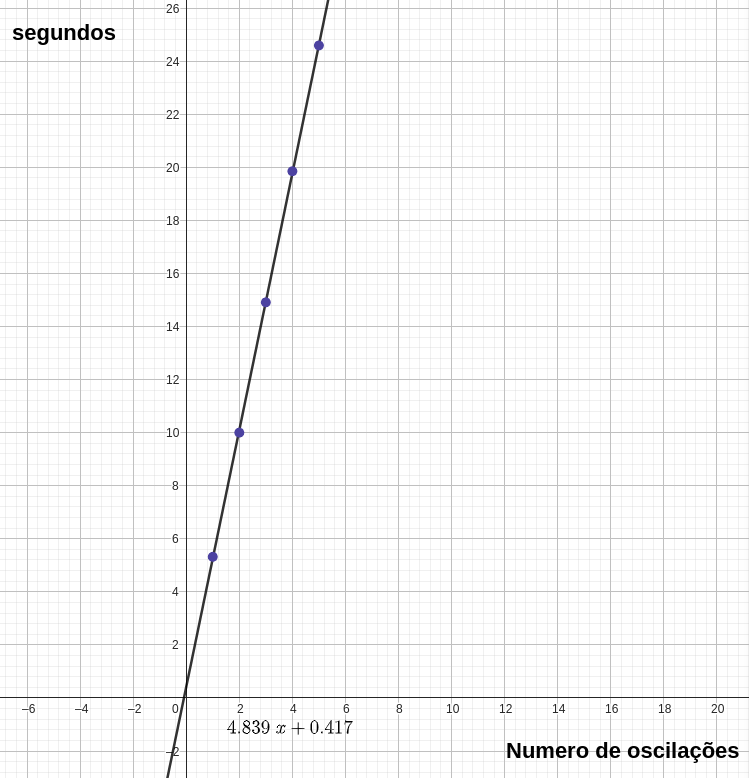
\includegraphics[width=0.35\linewidth]{fig/Torção no ar.png}
	\caption{Gráfico do numero de oscilações do pêndulo de torção no ar por tempo, tendo feita a regressão linear com 5 pontos}
	\label{Torçãonoar}
\end{figure}

\begin{figure}[H]
	\centering
	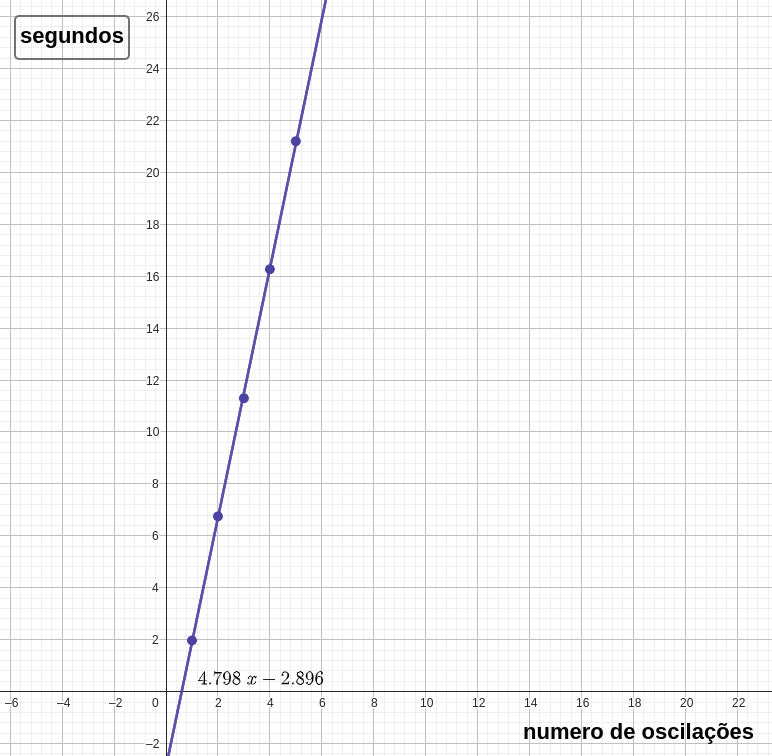
\includegraphics[width=0.35\linewidth]{fig/Oscilações no óleo.png}
	\caption{Gráfico do numero de oscilações do pêndulo de torção no óleo por tempo, tendo feita a regressão linear com 5 pontos}
	\label{Torçãonoóleo}
\end{figure}

Pêndulo no ar:
\begin{align*}
	f(x) &= 4,839x +  0,417 \text{ Sendo "f(x)" o tempo em segundos, e "x" o numero de oscilações} \\
 	f(x) &= 4,839 * 10 + 0,417\\
    f(x) &= \qty{48,807}{s}	
\end{align*}

Pêndulo no óleo:
\begin{align*}
	f(x) &= 4,798x -  2,896 \text{ Sendo "f(x)" o tempo em segundos, e "x" o numero de oscilações}\\
	f(x) &= 4,798 * 10 - 2,896\\
	f(x) &= \qty{45,084}{s}
\end{align*}

\begin{table}[H]
	\caption{Dados obtidos empiricamente do pêndulo de Torção no ar} \label{tabelaar}
	\begin{center}
		\begin{tabular}{c c c}
			\hline
			Oscilação & Tempo (s) & Variação do Tempo (s) \\
			\hline
			1 & 00:05.32 & 00:05.32\\
			2 & 00:10.00 & 00:04.68\\
			3 & 00:14.91 & 00:04.91\\
			4 & 00:19.85 & 00:04.94\\
			5 & 00:24.59 & 00:04.74\\
			6 & 00:29.50 & 00:04.91\\
			7 & 00:34.32 & 00:04.82\\
			8 & 00:39.24 & 00:04.92\\
			9 & 00:44.23 & 00:04.99\\
			10 & 00:48.94 & 00:04.71\\
			\hline
		\end{tabular}
	\end{center}
\end{table}

\begin{table}[H]
	\caption{Dados obtidos empiricamente do pêndulo de Torção no óleo} \label{tabelaóleo}
	\begin{center}
		\begin{tabular}{c c c}
			\hline
			Oscilação & Tempo (s) & Variação do Tempo (s) \\
			\hline
			1 & 00:01.97 & 00:01.97\\
			2 & 00:06.75 & 00:04.78\\
			3 & 00:11.30 & 00:04.55\\
			4 & 00:16.27 & 00:04.97\\
			5 & 00:21.20 & 00:04.93\\
			6 & 00:26.14 & 00:04.94\\
			7 & 00:31.08 & 00:04.94\\
			8 & 00:35.83 & 00:04.75\\
			9 & 00:40.42 & 00:04.59\\
			10 & 00:45.46 & 00:05.04\\
			\hline
		\end{tabular}
	\end{center}
\end{table}

Como observado nas tabelas \ref{tabelaar} e \ref{tabelaóleo}, as previsões da regressão linear estão de acordo com os valores empíricos. Além disso, a análise dos dados permite concluir que, no ar, o pêndulo apresentou oscilações com variações de tempo bastante regulares, com valor médio aproximado de \qty{4,86}{s} por oscilação. Isso sugere que, nesse meio de baixa resistência, o movimento mantém sua periodicidade e conserva energia por mais tempo.

Já no óleo, embora a média das oscilações também tenha se mantido próxima a \qty{4,85}{s}, a primeira oscilação foi significativamente mais curta (\qty{1,97}{s}), o que pode indicar um erro experimental ou falha na cronometragem. Ao desconsiderar essa medida inicial, a média passa para \qty{4,83}{s}, valor mais coerente com o esperado para um sistema amortecido.

Assim, ao excluir a primeira medição, conclui-se que o pêndulo no ar representa um sistema quase conservativo, enquanto o pêndulo no óleo evidencia a ação de um meio viscoso, que dissipa energia com mais intensidade, reduzindo a amplitude das oscilações com o tempo.




